\documentclass[floatsintext,man]{apa6}

\usepackage{amssymb,amsmath}
\usepackage{ifxetex,ifluatex}
\usepackage{fixltx2e} % provides \textsubscript
\ifnum 0\ifxetex 1\fi\ifluatex 1\fi=0 % if pdftex
  \usepackage[T1]{fontenc}
  \usepackage[utf8]{inputenc}
\else % if luatex or xelatex
  \ifxetex
    \usepackage{mathspec}
    \usepackage{xltxtra,xunicode}
  \else
    \usepackage{fontspec}
  \fi
  \defaultfontfeatures{Mapping=tex-text,Scale=MatchLowercase}
  \newcommand{\euro}{€}
\fi
% use upquote if available, for straight quotes in verbatim environments
\IfFileExists{upquote.sty}{\usepackage{upquote}}{}
% use microtype if available
\IfFileExists{microtype.sty}{\usepackage{microtype}}{}

% Table formatting
\usepackage{longtable, booktabs}
\usepackage{lscape}
% \usepackage[counterclockwise]{rotating}   % Landscape page setup for large tables
\usepackage{multirow}		% Table styling
\usepackage{tabularx}		% Control Column width
\usepackage[flushleft]{threeparttable}	% Allows for three part tables with a specified notes section
\usepackage{threeparttablex}            % Lets threeparttable work with longtable

% Create new environments so endfloat can handle them
% \newenvironment{ltable}
%   {\begin{landscape}\begin{center}\begin{threeparttable}}
%   {\end{threeparttable}\end{center}\end{landscape}}

\newenvironment{lltable}
  {\begin{landscape}\begin{center}\begin{ThreePartTable}}
  {\end{ThreePartTable}\end{center}\end{landscape}}




% The following enables adjusting longtable caption width to table width
% Solution found at http://golatex.de/longtable-mit-caption-so-breit-wie-die-tabelle-t15767.html
\makeatletter
\newcommand\LastLTentrywidth{1em}
\newlength\longtablewidth
\setlength{\longtablewidth}{1in}
\newcommand\getlongtablewidth{%
 \begingroup
  \ifcsname LT@\roman{LT@tables}\endcsname
  \global\longtablewidth=0pt
  \renewcommand\LT@entry[2]{\global\advance\longtablewidth by ##2\relax\gdef\LastLTentrywidth{##2}}%
  \@nameuse{LT@\roman{LT@tables}}%
  \fi
\endgroup}


  \usepackage{graphicx}
  \makeatletter
  \def\maxwidth{\ifdim\Gin@nat@width>\linewidth\linewidth\else\Gin@nat@width\fi}
  \def\maxheight{\ifdim\Gin@nat@height>\textheight\textheight\else\Gin@nat@height\fi}
  \makeatother
  % Scale images if necessary, so that they will not overflow the page
  % margins by default, and it is still possible to overwrite the defaults
  % using explicit options in \includegraphics[width, height, ...]{}
  \setkeys{Gin}{width=\maxwidth,height=\maxheight,keepaspectratio}
\ifxetex
  \usepackage[setpagesize=false, % page size defined by xetex
              unicode=false, % unicode breaks when used with xetex
              xetex]{hyperref}
\else
  \usepackage[unicode=true]{hyperref}
\fi
\hypersetup{breaklinks=true,
            pdfauthor={},
            pdftitle={Measuring Lay Theories of Parenting and Child Development},
            colorlinks=true,
            citecolor=blue,
            urlcolor=blue,
            linkcolor=black,
            pdfborder={0 0 0}}
\urlstyle{same}  % don't use monospace font for urls

\setlength{\parindent}{0pt}
%\setlength{\parskip}{0pt plus 0pt minus 0pt}

\setlength{\emergencystretch}{3em}  % prevent overfull lines


% Manuscript styling
\captionsetup{font=singlespacing,justification=justified}
\usepackage{csquotes}
\usepackage{upgreek}



\usepackage{tikz} % Variable definition to generate author note

% fix for \tightlist problem in pandoc 1.14
\providecommand{\tightlist}{%
  \setlength{\itemsep}{0pt}\setlength{\parskip}{0pt}}

% Essential manuscript parts
  \title{Measuring Lay Theories of Parenting and Child Development}

  \shorttitle{Measuring Parenting Theories}


  \author{Emily Hembacher\textsuperscript{1}~\& Michael C. Frank\textsuperscript{1}}

  % \def\affdep{{"", ""}}%
  % \def\affcity{{"", ""}}%

  \affiliation{
    \vspace{0.5cm}
          \textsuperscript{1} Stanford University  }

  \authornote{
    Add complete departmental affiliations for each author here. Each new
    line herein must be indented, like this line. Enter author note here.
    
    Correspondence concerning this article should be addressed to Michael C.
    Frank, 450 Serra Mall, Stanford, CA 94301. E-mail:
    \href{mailto:mcfrank@stanford.edu}{\nolinkurl{mcfrank@stanford.edu}}
  }


  \abstract{Enter abstract here. Each new line herein must be indented, like this
line.}
  \keywords{keywords \\

    \indent Word count: X
  }





\usepackage{amsthm}
\newtheorem{theorem}{Theorem}[section]
\newtheorem{lemma}{Lemma}[section]
\theoremstyle{definition}
\newtheorem{definition}{Definition}[section]
\newtheorem{corollary}{Corollary}[section]
\newtheorem{proposition}{Proposition}[section]
\theoremstyle{definition}
\newtheorem{example}{Example}[section]
\theoremstyle{definition}
\newtheorem{exercise}{Exercise}[section]
\theoremstyle{remark}
\newtheorem*{remark}{Remark}
\newtheorem*{solution}{Solution}
\begin{document}

\maketitle

\setcounter{secnumdepth}{0}



\section{Survey Construction}\label{survey-construction}

\subsection{Generation of items}\label{generation-of-items}

\subsection{Revised questionnaire
norming}\label{revised-questionnaire-norming}

\section{Survey Validation}\label{survey-validation}

\subsection{External Validity Study 1: Demographic
Factors}\label{external-validity-study-1-demographic-factors}

\begin{figure}
\centering
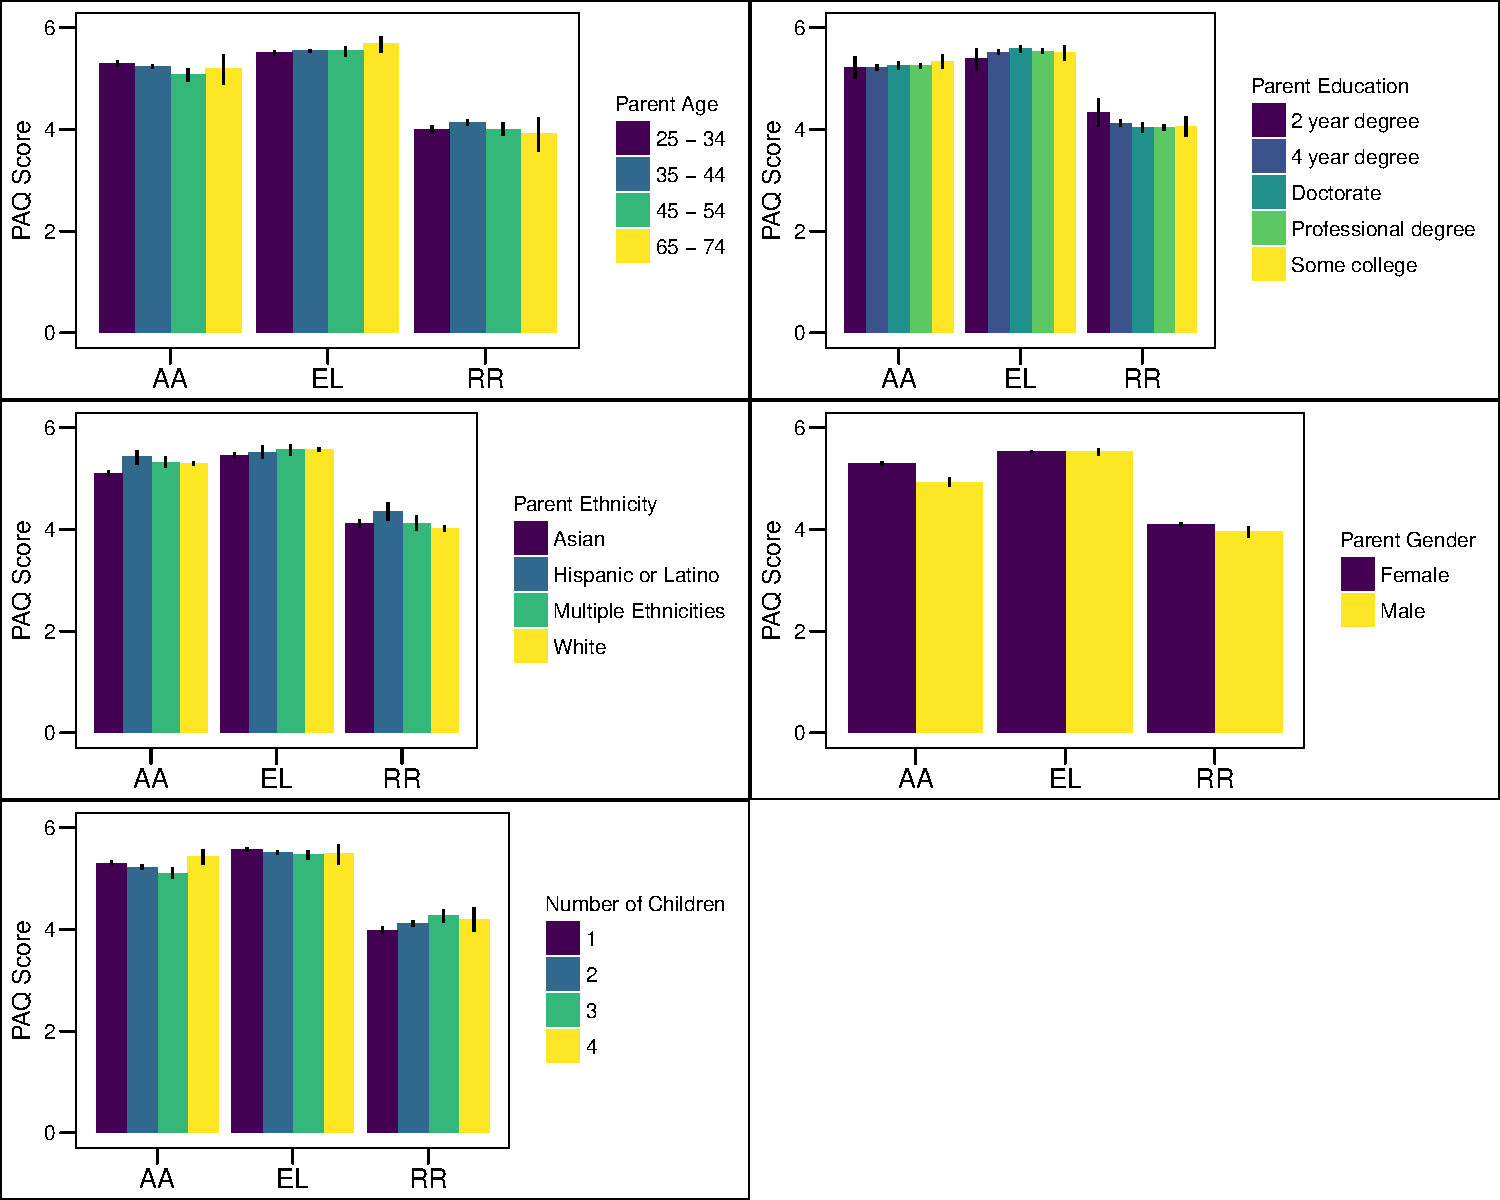
\includegraphics{PAQ_paper_files/figure-latex/demographics-1.pdf}
\caption{\label{fig:demographics}Demographic variability in PAQ scores.
Error bars represent +/-95\% CI computed by non-parametric bootstrap.}
\end{figure}

\begin{table}[h]
\centering
\begin{tabular}{llrrrr}
 Subscale & Factor & Estimate & Est. Error & Lower 95\% CI & Upper 95\% CI \\ 
  \hline
AA & Parent Age & -0.00 & 0.01 & -0.01 & 0.01 \\ 
   & Hispanic or Latino & 0.72 & 0.20 & 0.34 & 1.11 \\ 
   & Multiple Ethnicities & 0.50 & 0.16 & 0.18 & 0.82 \\ 
   & White & 0.31 & 0.09 & 0.12 & 0.49 \\ 
   & Parent Education & 0.02 & 0.02 & -0.01 & 0.05 \\ 
   & Number of children & -0.14 & 0.05 & -0.24 & -0.03 \\ 
   & Male & -0.70 & 0.11 & -0.92 & -0.48 \\ 
   \hline
EL & Parent Age & 0.01 & 0.01 & -0.00 & 0.02 \\ 
   & Hispanic or Latino & 0.26 & 0.19 & -0.12 & 0.64 \\ 
   & Multiple Ethnicities & 0.56 & 0.17 & 0.22 & 0.90 \\ 
   & White & 0.44 & 0.09 & 0.25 & 0.62 \\ 
   & Parent Education & 0.02 & 0.02 & -0.01 & 0.05 \\ 
   & Number of children & -0.14 & 0.05 & -0.24 & -0.03 \\ 
   & Male & -0.18 & 0.11 & -0.41 & 0.04 \\ 
   \hline
RR & Parent Age & -0.00 & 0.01 & -0.01 & 0.01 \\ 
   & Hispanic or Latino & 0.27 & 0.20 & -0.11 & 0.67 \\ 
   & Multiple Ethnicities & -0.02 & 0.17 & -0.34 & 0.31 \\ 
   & White & -0.20 & 0.10 & -0.38 & -0.01 \\ 
   & Parent Education & -0.02 & 0.02 & -0.05 & 0.01 \\ 
   & Number of children & 0.15 & 0.06 & 0.04 & 0.25 \\ 
   & Male & -0.17 & 0.12 & -0.39 & 0.06 \\ 
  \end{tabular}
\caption{Results of separate bayesian ordinal logistic regressionsof demographic factors on PAQ scores for each subscale.} 
\end{table}

Approaches to parenting are known to differ across cultures and groups.
To better understand whether the parenting attitudes captured by our
survey reflect group differences, we examined average scores on the PAQ
subscales based on demographic factors. We administered the PAQ to 680
parents who were members of a local children's museum and subsequently
asked them to provide information about their gender, level of
education, age, ethnicity, and the number of children they have. Figure
\ref{fig:demographics} displays the distributions of demographic
factors. To quantify any possible group differences, we fit Bayesian
mixed effects ordinal regression models for each subscale (AA, EL, RR)
with the following structure:

\texttt{agreement\ rating\ \textasciitilde{}\ age\ +\ education\ +\ ethnicity\ +\ gender\ +\ number\ of\ children\ +\ (1\ \textbar{}\ subject)\ +\ (1\textbar{}\ item)}

\subsection{Study 2: Relation to parenting
behaviors}\label{study-2-relation-to-parenting-behaviors}

One way of assessing the ecological validity of the PAQ is to ask
whether the parenting attitudes assessed by the current measure are
related to actual parenting behaviors. For example, do parents who
strongly agree with items on the Early Learning subscale read to their
children more often? Do parents who strongly endorse items on the Rules
and Respect subscale give more time-outs? To assess this, we asked
parents on mturk to rate the frequency with which they engaged in a
number of parenting behaviors after having filled out the PAQ.

\begin{figure}
\centering
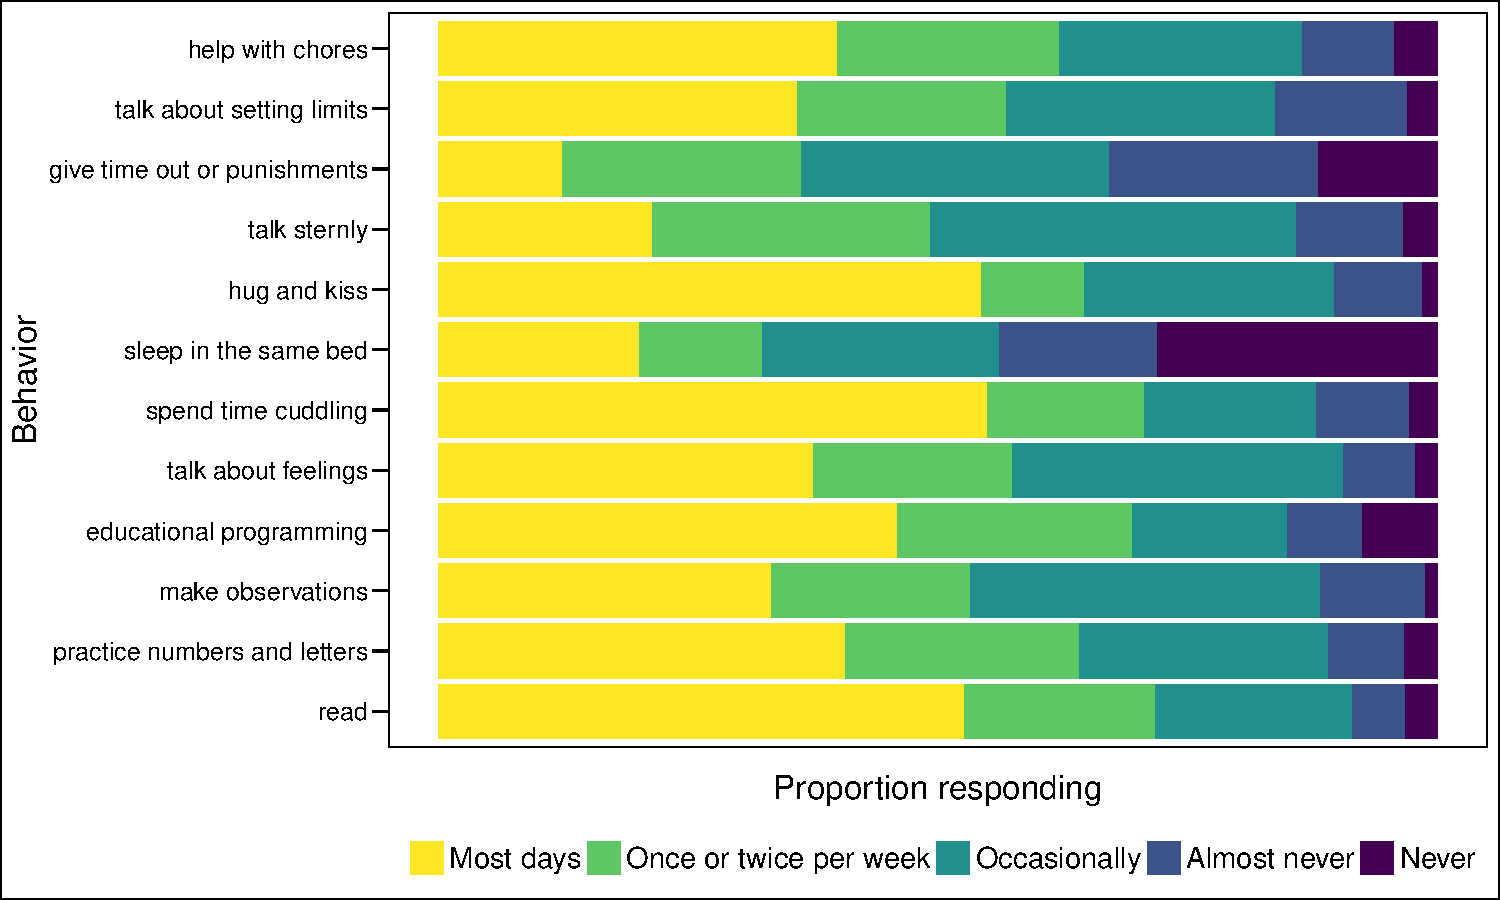
\includegraphics{PAQ_paper_files/figure-latex/behave_freq-1.pdf}
\caption{(\#fig:behave\_freq)Frequencies of different parenting
activities reported by parents.}
\end{figure}

\begin{figure}
\centering
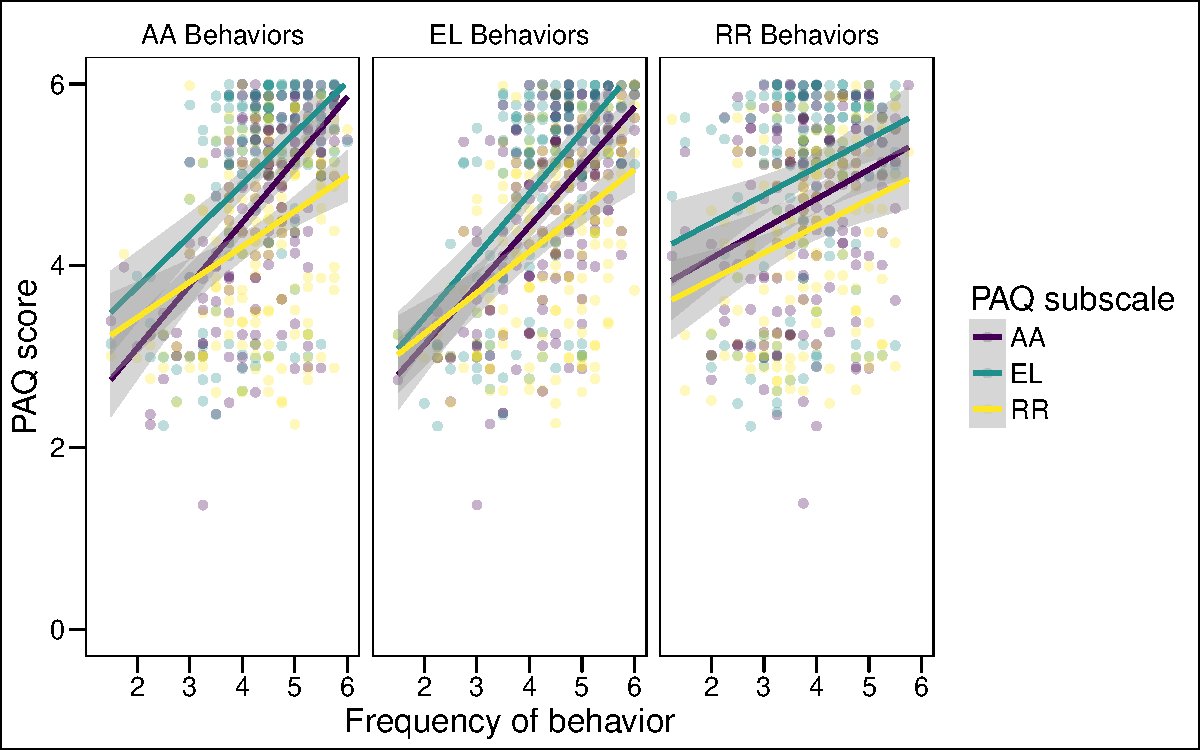
\includegraphics{PAQ_paper_files/figure-latex/behave_paq-1.pdf}
\caption{(\#fig:behave\_paq)Relations between PAQ scores (Affection and
Attachment, Early Learning, and Rules and Respect) and the frequency of
parenting behaviors divided into the same categories.}
\end{figure}

\begin{table}[h]
\centering
\begin{tabular}{llrrrr}
 Behavior Category & Factor & Estimate & Est.Error & l.95..CI & u.95..CI \\ 
  \hline
AA & AA PAQ score & 0.81 & 0.15 & 0.53 & 1.11 \\ 
   & RR PAQ score & -0.02 & 0.11 & -0.24 & 0.20 \\ 
   & EL PAQ score & -0.01 & 0.14 & -0.30 & 0.26 \\ 
   & Child Age & 0.01 & 0.01 & -0.00 & 0.02 \\ 
   \hline
EL & AA PAQ score & 0.36 & 0.18 & 0.01 & 0.73 \\ 
   & RR PAQ score & 0.20 & 0.14 & -0.07 & 0.47 \\ 
   & EL PAQ score & 0.52 & 0.18 & 0.17 & 0.88 \\ 
   & Child Age & 0.01 & 0.01 & -0.00 & 0.03 \\ 
   \hline
RR & AA PAQ score & 0.10 & 0.20 & -0.30 & 0.50 \\ 
   & RR PAQ score & 0.34 & 0.15 & 0.04 & 0.64 \\ 
   & EL PAQ score & 0.02 & 0.20 & -0.36 & 0.41 \\ 
   & Child Age & 0.03 & 0.01 & 0.01 & 0.05 \\ 
  \end{tabular}
\caption{Results of separate bayesian ordinal logistic regressions of PAQ scores and child age on frequency of parenting behaviors in Affection and Attachment (AA), Early Learning (EL), and Rules and Respect (RR) categories.} 
\end{table}

\subsection{Study 3: Uptake of new information about parenting and child
development}\label{study-3-uptake-of-new-information-about-parenting-and-child-development}

Parents' existing lay theories about parenting and child development may
be an important consideration for crafting interventions on parenting
behaviors. There have been frequent efforts to intervene on parenting
behaviors, for example, public service announcements telling parents to
read to their children; courses aimed at helping fathers engage with
their children; messages aimed at encouraging parents and teachers to
give children opportunities for free play. There is evidence that
existing lay theories can interact in surprising ways with this type of
messaging in other domains. How do parents' lay theories impact how they
uptake new information?

7.70\% of the data is excluded due to reading time exclusion.

The average accuracy for control questions was 0.76(CI = 0.73 - 0.78)
and the average accuracy for experimenter questions was 0.81(CI = 0.73 -
0.83). There was no significant difference in accuracy between
conditions, t = -4.83, p = 0.00.

\begin{figure}
\centering
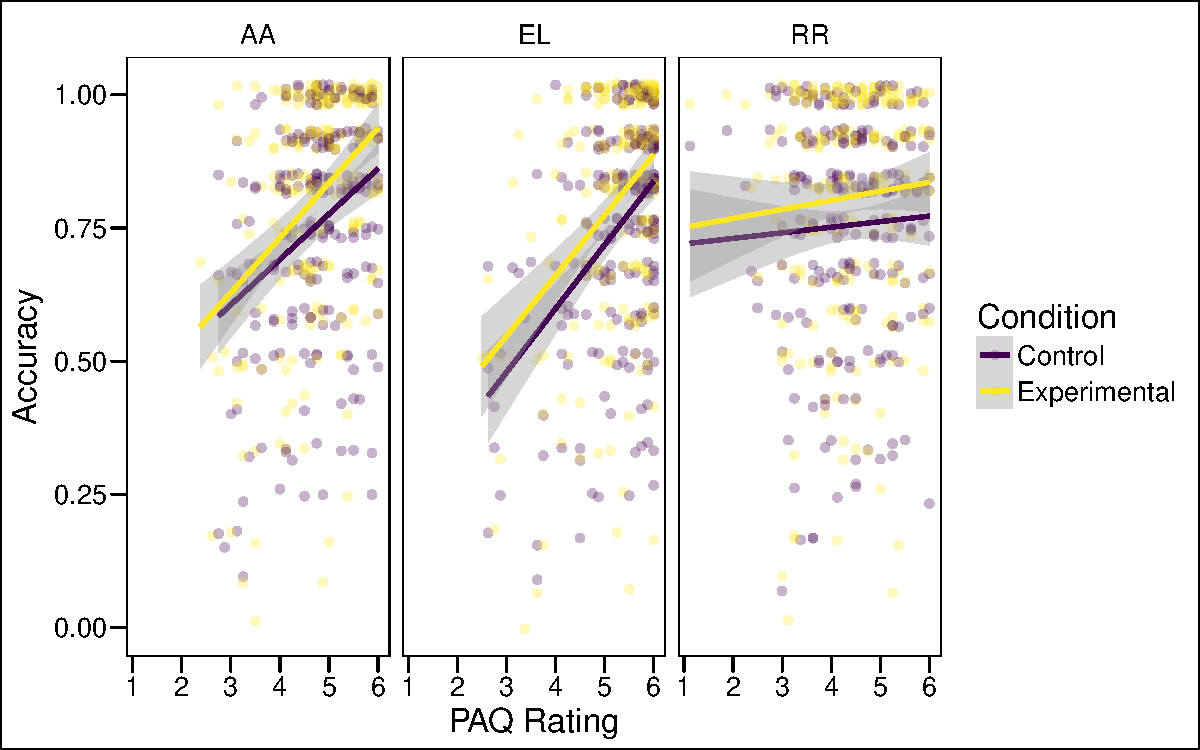
\includegraphics{PAQ_paper_files/figure-latex/uptake-1.pdf}
\caption{\label{fig:uptake}Relations between PAQ scores (Affection and
Attachment, Early Learning, and Rules and Respect) and the uptake of
information in experimental (child development-related) and control
articles.}
\end{figure}

\begin{table}[h]
\centering
\begin{tabular}{lrrrr}
  \hline
Factor & Estimate & Est. Error & Lower 95\% CI & Upper 95\% CI \\ 
  \hline
Condition & -0.21 & 0.75 & -1.68 & 1.29 \\ 
  AA PAQ score & 0.05 & 0.15 & -0.25 & 0.35 \\ 
  RR PAQ score & -0.21 & 0.11 & -0.42 & 0.01 \\ 
  EL PAQ score & 0.82 & 0.16 & 0.52 & 1.14 \\ 
  AA PAQ score * Condition & 0.42 & 0.16 & 0.11 & 0.73 \\ 
  RR PAQ score * Condition & 0.02 & 0.11 & -0.19 & 0.23 \\ 
  EL PAQ score * Condition & -0.27 & 0.16 & -0.58 & 0.05 \\ 
   \hline
\end{tabular}
\caption{Results of a bayesian logistic regression of PAQ scores and experimental condition on accuracy.} 
\end{table}

\newpage

\section{References}\label{references}

\begingroup
\setlength{\parindent}{-0.5in} \setlength{\leftskip}{0.5in}

\hypertarget{refs}{}

\endgroup






\end{document}
